% Draft manuscript - telemetry study only.  Compile with elsarticle (Overleaf: "Elsevier article").
% Numbers in the results sections are \input from paper/tables/*.tex, which
% scripts/build_paper_tables.py writes from the result files; do not type numbers by hand.
\documentclass[preprint,12pt,authoryear]{elsarticle}
\usepackage{amsmath,amssymb,booktabs,graphicx,url,siunitx,xcolor}
\usepackage[hidelinks]{hyperref}
\newcommand{\todo}[1]{\textcolor{red}{[TODO: #1]}}
\journal{Engineering Applications of Artificial Intelligence}

\begin{document}
\begin{frontmatter}
\title{Alarm selection, not deep event scoring, decides spacecraft telemetry alarm quality:
a pre-registered study on the full ESA-ADB missions}

\author[aff1]{\todo{Author names, ORCID}}
\affiliation[aff1]{organization={\todo{Affiliation}}, country={\todo{Country}}}

\begin{abstract}
On the full channel sets of the ESA Anomaly Detection Benchmark (58 and 47 monitored
channels), published detectors score below 0.08 on the benchmark's primary metric, the
corrected event-wise $F_{0.5}$. We ask whether this reflects the detectors or the way their
alarms are selected. We introduce an out-of-fold protocol for the official split: every
training sample is scored by a model that never saw it, so the alarm layer can be selected on
all training labels (109 events on Mission~1, against 9 in the usual calibration window).
The alarm layer is event-level and conformal: per-channel conformal p-values,
Benjamini--Hochberg across channels, persistence and merging.

We pre-registered and hash-froze three hypotheses on Mission~1, the primary mission, and
scored each arm on the test half once:
\begin{itemize}
\item \textbf{Selection (supported).} Selecting the layer on the whole training half raised
  an AR(8) forecaster from 0.074 to 0.428 (difference $+0.353$, 95\,\% CI
  $[+0.206,+0.488]$, Holm $p=0.0015$).
\item \textbf{Deep scorer against the forecaster (refuted).} A supervised, causal temporal
  convolutional event scorer trained out of fold reached $0.205\pm0.114$ (5 seeds), below
  the AR(8) arm ($-0.222$, $[-0.395,+0.042]$).
\item \textbf{Deep scorer against trees (refuted).} The same scorer was also below
  gradient-boosted trees on identical features ($0.544\pm0.236$; $-0.338$,
  $[-0.540,-0.033]$).
\end{itemize}

Mission~2 is close to saturated: a parameter-free out-of-limit rule scores 0.894 there. In
the Mission~2 replication, selection on the whole training half was \emph{worse} than the
calibration window ($-0.089$, $[-0.143,-0.049]$). A point-level adaptive conformal
comparator scored at most 0.002 on every score source of both missions. On the same
full-channel scores, the event-level layer scored 0.21--0.90 (seed means).

Exploratory diagnostics trace the deep scorer's failure to a shift between train and test in
its nominal score distribution: nominal test samples exceed the calibration quantile 3--54
times more often than in cross-validation, against 0.8 times for AR(8). Under an
operator-grade metric, how the alarm layer is selected and how stable the scorer's nominal
distribution is matter more than model capacity.
\end{abstract}

\begin{keyword}
spacecraft telemetry \sep anomaly detection \sep conformal prediction \sep false discovery
rate \sep temporal convolutional network \sep ESA-ADB \sep pre-registration
\end{keyword}
\end{frontmatter}

% =====================================================================================
\section{Introduction}\label{sec:intro}

Spacecraft operators review telemetry alarms by hand. A monitor is useful only if its alarms
are few, mostly correct and timely. The European Space Agency Anomaly Detection Benchmark
(ESA-ADB) \citep{kotowski2026esaadb} encodes this requirement in its primary metric. That
metric is an event-wise $F_{0.5}$ score whose precision is additionally multiplied by the
true-negative rate. Under this metric, and on the full sets of 58 and 47 monitored channels
of its two benchmark missions, no published baseline exceeds 0.08.
\citet{kotowski2026esaadb} attribute the failure to thresholding and post-processing rather
than to the detectors themselves.

Recent work has attacked the problem from several directions:
\begin{itemize}
\item similarity-search and Gaussian-process detectors with adaptive retraining
  \citep{brancato2027ast};
\item monthly incremental retraining with extreme-value thresholds under a non-official
  chronological protocol \citep{alcarria2026};
\item supervised ensembles on the challenge split of Mission~1 \citep{allegrini2026};
\item workload-constrained alerting policies \citep{heydari2026};
\item a pre-registered study of telecommand conditioning, adaptive conformal thresholds and
  operator deferral \citep{sahin2026tccad}.
\end{itemize}
The last study reports that per-channel, point-level conformal thresholds calibrate the
point-wise false-alarm rate. On Mission~1, however, they lower the anomaly event-wise
$F_{0.5}$ to the order of $10^{-5}$, because they produce millions of alarm events.

This paper starts from a simple observation. In our earlier exploratory study, the same
forecaster and alarm layer that scored 0.96 on Mission~2 scored 0.07 on Mission~1. The
alarm layer had been selected on a 9-month window of the training half that holds only 9
labelled events. We ask two questions:
\begin{enumerate}
\item Does selecting the alarm layer on out-of-fold scores of the \emph{whole} training half
  (109 labelled events on Mission~1) change the picture?
\item Does a supervised deep event scorer, trained out of fold on those labels, add to an
  unsupervised forecaster once both feed the same event-level conformal alarm layer?
\end{enumerate}

\paragraph{Contributions}
\begin{enumerate}
\item An out-of-fold protocol for the official ESA-ADB split. It scores every training sample
  with a model that did not see it, so alarm selection and supervised training can use all
  training labels while the test half stays untouched (Section~\ref{sec:oof}).
\item A causal, channel-shared temporal convolutional event scorer with cross-channel mixing,
  trained on forecast residuals and telemetry (Section~\ref{sec:model}). It is paired with an
  event-level conformal false-discovery-rate alarm layer (Section~\ref{sec:alarm}).
\item A pre-registered, hash-frozen confirmatory evaluation on both missions at full channel
  scale. It includes strong label-free baselines (out-of-limit, GlobalSTD), gradient-boosted
  trees on identical features, and a point-level adaptive conformal comparator
  (Sections~\ref{sec:design}--\ref{sec:results}).
\item The evidence on what matters (Section~\ref{sec:discussion}):
  \begin{itemize}
  \item Alarm selection on Mission~1 is supported.
  \item The deep scorer is refuted against both simpler scorers.
  \item Whole-half selection reverses on Mission~2.
  \item Event-level calibration is necessary; point-level calibration fails.
  \item An exploratory diagnostic locates the deep scorer's failure in the
    train-to-test drift of its nominal scores.
  \end{itemize}
\end{enumerate}

% =====================================================================================
\section{Related work}\label{sec:related}
\paragraph{Spacecraft telemetry benchmarks}
\citet{hundman2018} introduced LSTM forecasting with non-parametric dynamic thresholds on
SMAP/MSL. Those benchmarks were later shown to be flawed \citep{wu2021flawed}, and
point-adjusted metrics inflate scores \citep{kim2022rigorous}. ESA-ADB
\citep{kotowski2026esaadb} replaces them with three missions annotated by spacecraft
operations engineers and with a hierarchy of event-wise, channel-aware, timing and
affiliation metrics. OPS-SAT-AD \citep{ruszczak2025opssat} provides labelled fragments for
supervised classification.

\paragraph{Recent ESA-ADB results}
Reported Mission~1 full-channel scores range from 0.061 \citep{kotowski2026esaadb} to 0.902
\citep{brancato2027ast}, and the protocols differ. \citet{alcarria2026} report 0.700 and
0.698 under monthly retraining over each whole mission. They also cite 0.424 and 0.882 for
the PitIA system under a static split \citep{tejedor2025pitia}. \citet{allegrini2026} report
0.853 on the private leaderboard of the Kaggle challenge, which uses a different test split
and does not separate anomalies from rare events. \citet{nguyen2026} compare supervised and
unsupervised models with uncorrected metrics, mostly on lightweight subsets.
\todo{Read Brancato et al.\ (2027) in full and state their exact protocol. Their
out-of-limit reference (0.754 on Mission~1) is far above what an out-of-limit rule achieves
under our implementation of the official protocol (0.005); see Table~\ref{tab:baselines}.}

\paragraph{Thresholds, conformal inference and false-alarm control}
Extreme-value thresholds \citep{siffer2017} and dynamic thresholds \citep{hundman2018} are
standard. Conformal p-values against nominal calibration scores, combined with the
Benjamini--Hochberg procedure \citep{benjamini1995}, control the marginal false discovery
rate under exchangeability \citep{bates2023}. Weighted and adaptive variants address drift
\citep{barber2023,gibbs2021aci}. \citet{sahin2026tccad} apply split, sliding and adaptive
conformal thresholds per channel and per point. We instead test across channels at every
step and require persistence before an alarm event is raised. Section~\ref{sec:results}
compares the two layers on identical scores.

\paragraph{Telecommands}
\citet{sahin2026tccad} report a pre-registered negative result for telecommand conditioning.
Our exploratory study reached the same conclusion with forecasters (Appendix~\ref{app:explo}).
Telecommands are therefore not used in this paper.

% =====================================================================================
\section{Data and evaluation protocol}\label{sec:data}
We use the ESA Anomalies Dataset v1.0 (Zenodo 12528696). Missions~1 and~2 are resampled to
the official 30\,s and 18\,s zero-order-hold grids, following the official preprocessing
(monotonic-channel differencing and restoration of annotated samples). The split is the
official one: training up to 2007-01-01 for Mission~1 and 2001-10-01 for Mission~2, testing
afterwards. All 58 and 47 target channels are used. A literal port of the official pandas
preprocessing reproduces our vectorised grids exactly (unit test in the repository). The
official GlobalSTD baseline, run through our pipeline, reproduces the published primary
metric in all eight mission, channel-set and threshold configurations
(Table~\ref{tab:baselines}).

\paragraph{Metric}
The primary metric is the official corrected event-wise $F_{0.5}$ over anomalies and rare
nominal events. Writing $TP_e$ and $FN_e$ for detected and missed labelled events, $FP_e$
for predicted alarm events that overlap no label, and $\mathrm{TNR}$ for the sample-wise
true-negative rate,
\begin{equation}
  P_e = \frac{TP_e}{TP_e+FP_e}\cdot \mathrm{TNR},\qquad R_e=\frac{TP_e}{TP_e+FN_e},\qquad
  F_{0.5}=\frac{1.25\,P_eR_e}{0.25\,P_e+R_e}.
\end{equation}
We use the official metric code unchanged. Secondary metrics are:
\begin{itemize}
\item the anomaly-only event-wise $F_{0.5}$;
\item false alarms per year (alarm runs that touch no label);
\item alarm runs that touch only rare nominal events;
\item ADTQC detection timing;
\item affiliation $F_{0.5}$.
\end{itemize}

\paragraph{Labelled events}
The Mission~1 training half holds 63 anomalies and 42 rare nominal events (all channels).
Its test half holds 55 and 36. Thirteen of the 17 event classes in the test half also occur
in the training half. Mission~2 holds 25 anomalies and 257 rare events in training, and 6
anomalies and 356 rare events in test. Mission~2 is close to saturated by a parameter-free
out-of-limit rule (Table~\ref{tab:baselines}), so Mission~1 is the primary mission and
Mission~2 a replication.

% =====================================================================================
\section{Method}\label{sec:method}
\subsection{Out-of-fold residual scores}\label{sec:oof}
Let $z_{t,c}$ be the robust-normalised value of channel $c$ at grid step $t$. We use the
training-half median and interquartile range of nominal samples.
\begin{itemize}
\item The training half is cut into $K=5$ contiguous blocks.
\item For block $b$, a ridge AR(8) forecaster is fitted on the nominal samples of the other
  blocks, excluding one day on either side of $b$. It produces iterated 16-step forecasts
  $\hat z_{t,c}$ inside $b$.
\item The non-conformity score is $s_{t,c}=|z_{t,c}-\hat z_{t,c}|/\sigma_c$, where
  $\sigma_c$ is a robust residual scale estimated on the fitting blocks.
\item Test scores come from an AR(8) fitted on all nominal training samples.
\end{itemize}
AR(8) was the strongest encoder in our exploratory comparison with persistence, a causal TCN,
PatchTST \citep{nie2023patchtst} and Chronos-Bolt \citep{ansari2024chronos}
(Appendix~\ref{app:explo}).

\subsection{Supervised event scorer}\label{sec:model}
Each channel and step receives seven causal features:
\begin{itemize}
\item $\operatorname{asinh} z$;
\item $\log(1+s)$;
\item its trailing exponential means with time constants 1\,h, 12\,h and 3\,d;
\item $\operatorname{asinh}(z-\bar z^{1\mathrm{d}})$, the value minus its trailing 1-day
  mean;
\item a forecast-availability flag.
\end{itemize}
The scorer is a causal dilated temporal convolutional network \citep{bai2018tcn}. It has 8
levels with two convolutions each, kernel 3, width 64, and a receptive field of 1{,}021
steps. All channels share its weights; it adds a learned channel embedding and, every two
levels, mixes channels in a permutation-equivariant way (the channel mean is projected and
added back). A $1\times1$ head outputs three logits per channel and step: nominal, anomaly
and rare nominal event. Training uses class-weighted cross-entropy with weights 1, 5 and 5;
communication gaps are ignored. Each run takes 1{,}500 AdamW steps on windows of 2{,}048
steps with all channels, half of them centred on labelled samples, under a one-cycle
schedule. The event score is the log-odds of ``anomaly or rare event'' against ``nominal''.
The scorer is trained out of fold on the same blocks: one model per held-out block, and a
final model on all blocks for the test half. A unit test checks that it is causal: a change
at step $t$ leaves every output before $t$ unchanged.

\paragraph{Tree baseline}
A 3-class XGBoost model \citep{chen2016xgboost} uses the same seven features, plus trailing
maxima of $\log(1+s)$ over 16 and 256 steps and the channel index. It has 400 trees of depth
8, is trained on $2\times10^{6}$ subsampled rows (half of them labelled), and follows the
same out-of-fold protocol.

\subsection{Event-level conformal alarm layer}\label{sec:alarm}
For any score source, each channel's nominal out-of-fold training scores form a calibration
pool. A test score receives the conformal p-value
$p_{t,c}=(1+\#\{\text{pool}\ge s_{t,c}\})/(n_c+1)$. At each step the Benjamini--Hochberg
procedure at level $q$ is applied across channels \citep{bates2023,benjamini1995}. A global
alarm requires $k$ consecutive steps with at least one rejected channel. Alarm runs closer
than 1\,h are merged, and the reported channels are those rejected inside the run. Two
variants are also evaluated: a per-channel quantile threshold, and a rolling variant whose
pool is refreshed daily from the trailing 30 days of unlabelled test scores. Serial
dependence and drift violate exchangeability, so $q$ is treated as a tuning parameter and
realised false-alarm rates are reported.

\paragraph{Selection}
The level $q\in\{10^{-2},10^{-3},10^{-4},10^{-5}\}$ and the persistence
$k\in\{1,3,10,30,100\}$ are chosen by cross-fitting over the two halves of the training
half. The layer is calibrated on one half, alarms are raised on the other, and the official
metric is computed on that half's labels; the two directions are averaged. The chosen layer
is refitted on the whole training half and applied once to the test half.

\paragraph{Point-level comparator}
The comparator is per-channel adaptive conformal inference \citep{gibbs2021aci} with target
$\alpha=0.01$ and $\gamma\in\{0.001,0.005,0.01,0.05\}$. As in \citet{sahin2026tccad},
$\gamma$ is chosen as the value whose nominal false-alarm rate on the second training half is
closest to $\alpha$. The global alarm is the OR over channels. It is evaluated without
persistence or merging, and also with our event logic.

% =====================================================================================
\section{Experimental design}\label{sec:design}
The analysis was pre-registered and frozen before any test-half number of the arms below
existed. The freeze consists of SHA-256 hashes of 28 code and protocol files
(freeze ID \texttt{09a98f5e160e}), and the test-scoring code refuses to run if any of them
has changed. Table~\ref{tab:arms} lists the arms:
\begin{itemize}
\item A0: AR(8), alarm layer selected on the 9-month calibration window;
\item A1: AR(8), out of fold, layer selected on the whole training half;
\item A2: XGBoost event scorer;
\item A3: TCN event scorer.
\end{itemize}
A2 and A3 use 5 seeds each.

The confirmatory family on Mission~1 is:
\begin{itemize}
\item H4: A3 $>$ A1;
\item H5: A3 $>$ A2;
\item H6: A1 $>$ A0.
\end{itemize}
Each comparison uses the primary metric and the conformal-BH layer. It is tested by a paired
moving-block bootstrap \citep{kunsch1989}: 30-day blocks are shared by both arms, seeds are
resampled hierarchically, and there are 2{,}000 replicates. The family is corrected by Holm
\citep{holm1979}. The minimum effect size of interest is 0.05. A hypothesis is
\emph{supported} if its Holm-adjusted $p<0.05$ and its estimate is at least 0.05. It is
\emph{refuted} if its 95\,\% interval lies below 0.05. Otherwise it is \emph{inconclusive}.
Mission~2 repeats the same tests as a replication, without inference.

% =====================================================================================
\section{Results}\label{sec:results}
\subsection{Reproduction and label-free baselines}
Table~\ref{tab:baselines} lists the baselines.
\begin{itemize}
\item \textbf{Reproduction.} The official GlobalSTD detector, run through our preprocessing
  and metric adapter, reproduces the published primary metric to its printed precision in
  all eight configurations.
\item \textbf{Mission~1.} Every label-free rule fails on the full Mission~1 channel set
  ($\le0.005$).
\item \textbf{Mission~2.} An out-of-limit rule alarms whenever a sample leaves the range of
  its channel's nominal training samples. It has no free parameter, yet it scores 0.894 on
  the full Mission~2 set and 0.965 on its lightweight subset. Both are above every
  published DMLR value.
\end{itemize}
The second point is why Mission~2 was pre-registered as a replication rather than as the
primary mission.
\IfFileExists{tables/baselines.tex}{\begin{table}[t]\centering\small
\caption{Corrected event-wise $F_{0.5}$ (anomalies and rare events) on the official test halves. GlobalSTD rows show our run and, in parentheses, the value published in DMLR Table~4. $^\dagger$Exploratory: selected on the last 9 months of the training half.}\label{tab:baselines}
\begin{tabular}{lcccc}\toprule
 & \multicolumn{2}{c}{Mission 1} & \multicolumn{2}{c}{Mission 2}\\
\cmidrule(lr){2-3}\cmidrule(lr){4-5}
Detector & full (58) & lightweight & full (47) & lightweight\\\midrule
Best published (DMLR) & 0.061 & 0.786 & 0.079 & 0.949\\
GlobalSTD3 (official) & 0.0004 (<0.001) & 0.0011 (0.001) & 0.0075 (0.008) & 0.0071 (0.007)\\
GlobalSTD5 (official) & 0.0029 (0.003) & 0.253 (0.253) & 0.063 (0.064) & 0.075 (0.075)\\
Out-of-limit, nominal training range & 0.0007 & 0.202 & 0.894 & 0.965\\
Out-of-limit, full training range & 0.0051 & 0.000 & 0.261 & 0.080\\
COSMOS monitor (AR(8), EWMA, fixed rule) & 0.0038 & 0.202 & 0.047 & 0.788\\
A0: AR(8) + conformal-BH, 9-month selection$^\dagger$ & 0.074 & 0.408 & 0.962 & 0.908\\
\bottomrule\end{tabular}\end{table}
}{}
\IfFileExists{tables/arms.tex}{\begin{table}[t]\centering\small
\caption{Pre-registered arms (freeze \texttt{09a98f5e160e}). All share the alarm layer of
Section~\ref{sec:alarm}.}\label{tab:arms}
\begin{tabular}{llll}\toprule
Arm & Scores & Selection of $(q,k)$ & Seeds\\\midrule
A0 & AR(8), fitted on 2000--2005 (M1) & cross-fit on 9-month calibration window & --\\
A1 & AR(8), out of fold ($K=5$) & cross-fit on whole training half & --\\
A2 & XGBoost event scorer, out of fold & cross-fit on whole training half & 5\\
A3 & TCN event scorer, out of fold & cross-fit on whole training half & 5\\
\bottomrule\end{tabular}\end{table}
}{}

\subsection{Confirmatory comparisons (Mission 1)}
Table~\ref{tab:confirmatory} and Fig.~\ref{fig:arms} give the pre-registered outcomes.

\paragraph{H6 is supported}
With alarm selection on the whole training half, the same AR(8) scores raise the primary
metric from 0.074 to 0.428 (difference $+0.353$, 95\,\% CI $[+0.206,+0.488]$, Holm
$p=0.0015$).
\begin{itemize}
\item False alarms fall from 92 to 1.1 per year.
\item The selected layer is strict ($q=10^{-4}$, $k=10$), with precision 0.667 and recall
  0.176.
\end{itemize}

\paragraph{H4 and H5 are refuted}
The supervised TCN event scorer reaches $0.205\pm0.114$ over 5 seeds.
\begin{itemize}
\item Against AR(8) the difference is $-0.222$, $[-0.395,+0.042]$. The upper bound is below
  the 0.05 minimum effect, so the pre-registered verdict is ``refuted'', although the
  Holm-adjusted $p=0.10$.
\item Against gradient-boosted trees on identical features ($0.544\pm0.236$) the difference
  is $-0.338$, $[-0.540,-0.033]$.
\end{itemize}
The TCN raises 20.9 false alarms per year on average, against 8.5 for the trees and 1.1 for
AR(8).

\paragraph{Training-half cross-validation versus test}
The cross-validated training-half score, the selection objective, overstated test
performance for every arm, and most for the TCN. It was 0.624 for AR(8) and 0.70--0.77 for
the trees, against $0.536$ on average for the TCN (seed range 0.35--0.65).
\IfFileExists{tables/confirmatory.tex}{\begin{table}[t]\centering\small
\caption{Confirmatory comparisons, primary metric, conformal-BH layer. Values are official seed means; the interval and $p$ come from the paired hierarchical block bootstrap. Mission~1 is the pre-registered family (Holm); Mission~2 is a replication.}\label{tab:confirmatory}
\begin{tabular}{llcccccl}\toprule
Mission & Test & A & B & $\Delta$ & 95\,\% CI & $p_{\mathrm{Holm}}$ & Verdict\\\midrule
1 & H4 & 0.205 & 0.428 & -0.222 & [-0.395, +0.042] & 0.1010 & refuted\\
1 & H5 & 0.205 & 0.544 & -0.338 & [-0.540, -0.033] & 0.0700 & refuted\\
1 & H6 & 0.428 & 0.074 & +0.353 & [+0.206, +0.488] & 0.0015 & supported\\
2 & H4 & 0.875 & 0.874 & +0.001 & [-0.055, +0.054] & -- & replication (no inference)\\
2 & H5 & 0.875 & 0.904 & -0.029 & [-0.103, +0.037] & -- & replication (no inference)\\
2 & H6 & 0.874 & 0.962 & -0.089 & [-0.143, -0.049] & -- & replication (no inference)\\
\bottomrule\end{tabular}\end{table}
}{}
\begin{figure}[t]\centering
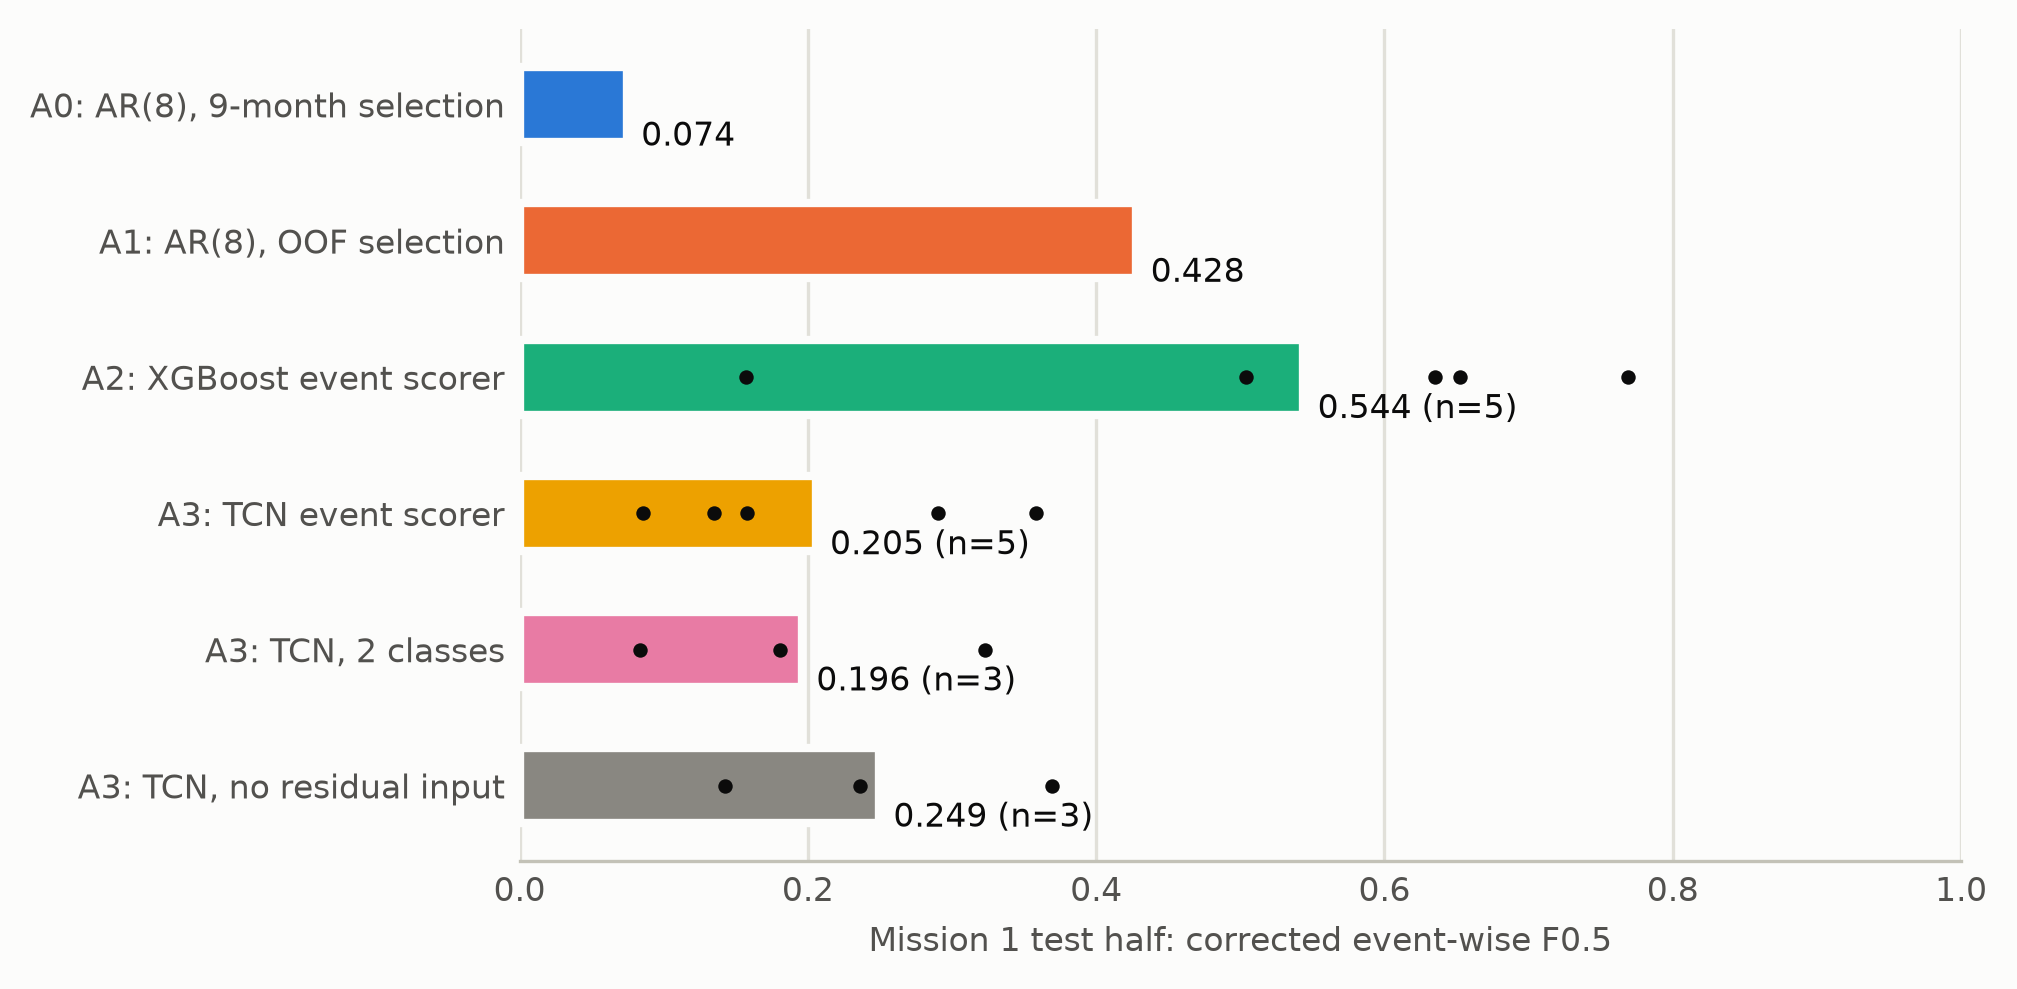
\includegraphics[width=0.85\linewidth]{figures/test_arms_m1.png}
\caption{Mission~1 test half, primary metric, conformal-BH layer. Bars show seed means and
dots individual seeds. A0 and A1 are deterministic.}\label{fig:arms}
\end{figure}
\begin{figure}[t]\centering
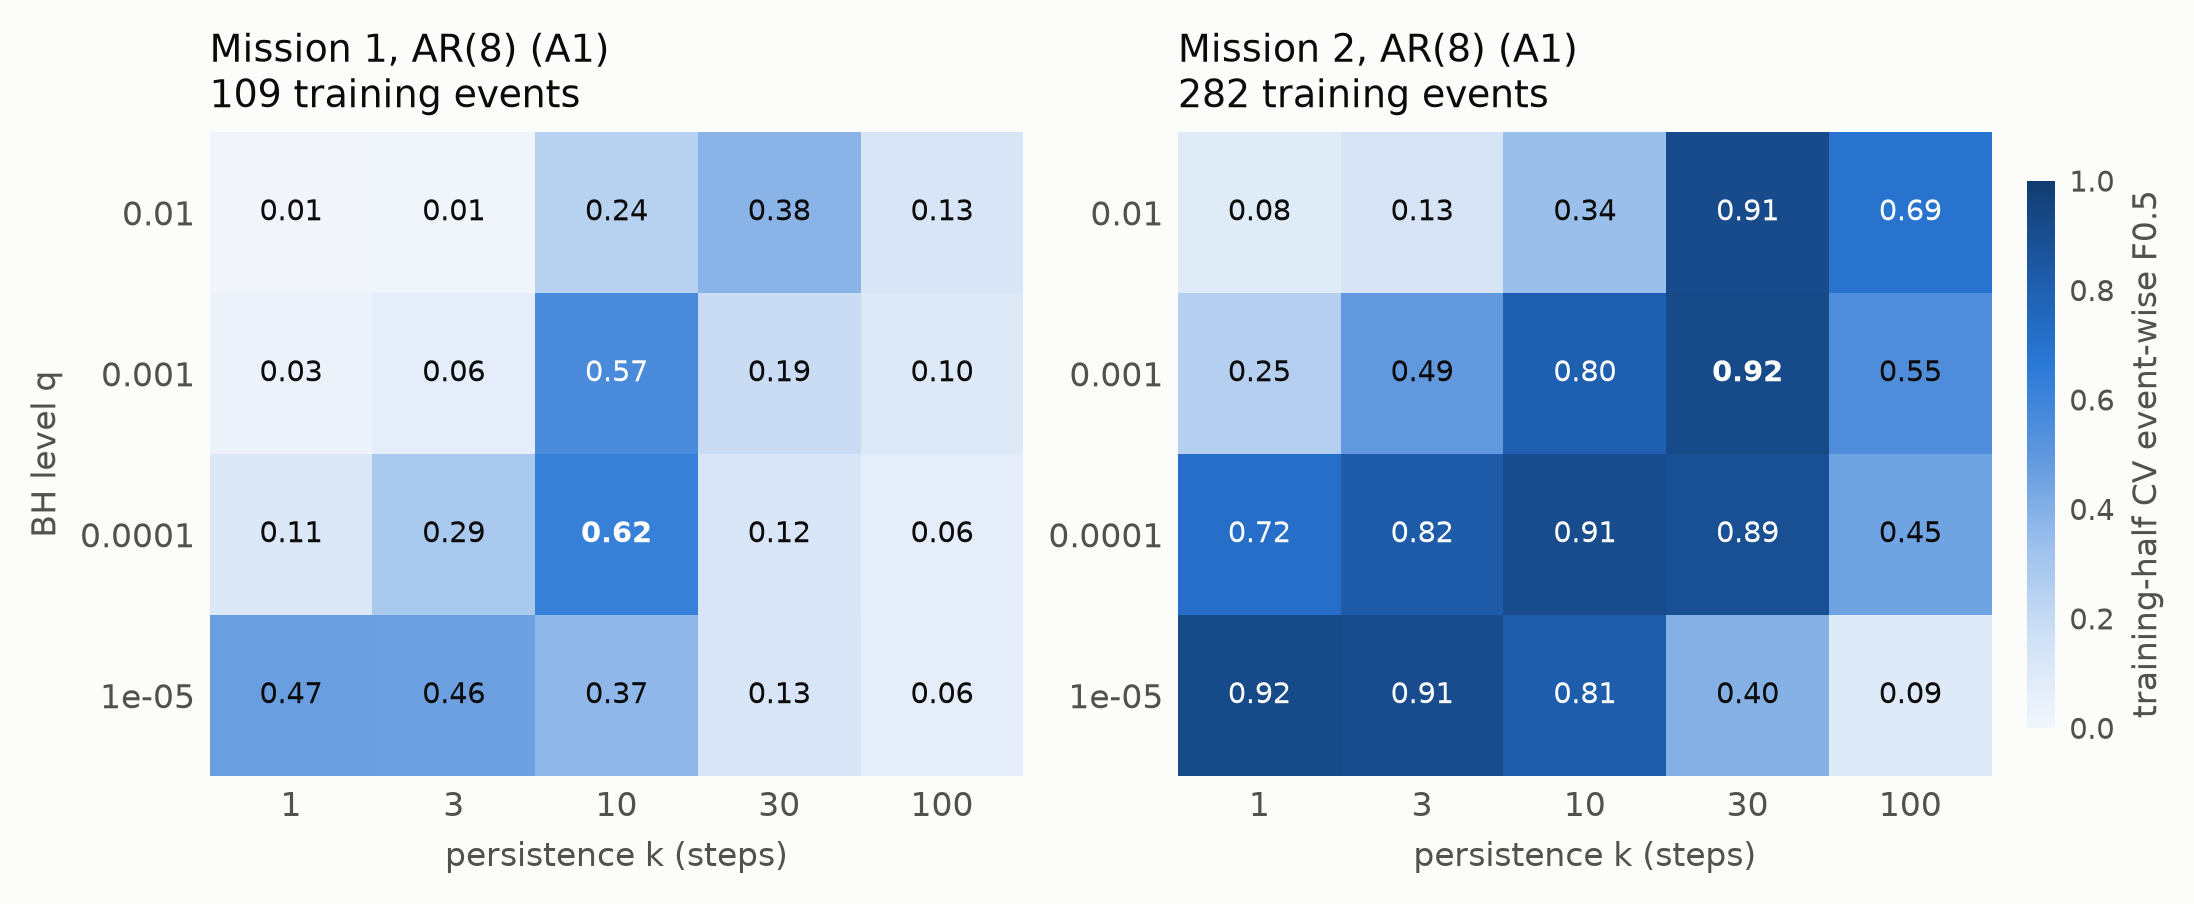
\includegraphics[width=0.95\linewidth]{figures/selection_landscape.png}
\caption{Cross-validated training-half event-wise $F_{0.5}$ of AR(8) scores over the
selection grid. Training labels only. The Mission~1 optimum is a narrow ridge at $k=10$;
Mission~2 has a broad plateau.}\label{fig:landscape}
\end{figure}

\subsection{Replication (Mission 2)}
On Mission~2 the three arms are statistically indistinguishable:
\begin{itemize}
\item A1 (AR(8)) 0.874;
\item A2 (trees) $0.904\pm0.050$;
\item A3 (TCN) $0.875\pm0.058$.
\end{itemize}
Selection on the whole training half was worse than the 4.5-month calibration window
($0.874$ against $0.962$; $-0.089$, $[-0.143,-0.049]$). The selection effect therefore does
\emph{not} replicate. It helps where the recent window holds too few events to select from
(Mission~1) and hurts where the recent window is representative of the test period
(Mission~2; Fig.~\ref{fig:landscape} shows its broad optimum). On the lightweight subsets,
A1 reaches 0.978 on Mission~2 but only 0.025 on Mission~1 with conformal-BH (0.350 with the
threshold layer).

\subsection{Alarm layers, ablations and the point-level comparator}
Table~\ref{tab:ablations} reports every secondary layer and ablation.
\begin{itemize}
\item \textbf{Point-level ACI.} Per-channel adaptive conformal inference (target
  $\alpha=0.01$) holds its point-wise false-alarm rate on the test half (0.0098--0.0100),
  as intended. Its primary metric is nevertheless $\le0.002$ for every score source, because it
  raises up to $1.6\times10^6$ alarm runs. Adding our persistence and merging lifts it only to
  at most 0.05.
\item \textbf{Event-level layer.} On the same full-channel scores, the layer selected on
  the training half reaches 0.21--0.90 (seed means).
\item \textbf{TCN ablations.} Removing the residual inputs ($0.249\pm0.114$, $n=3$) or
  merging the two event classes ($0.196\pm0.120$, $n=3$) changes the TCN by less than its
  seed spread.
\item \textbf{Calibrator.} The per-channel threshold layer is the best layer for the trees on
  Mission~1 ($0.613\pm0.159$) and for AR(8) on Mission~2 (0.977).
\end{itemize}
\IfFileExists{tables/ablations.tex}{\begin{table}[t]\centering\scriptsize
\caption{Test-half corrected event-wise $F_{0.5}$ for every arm and alarm layer (mean $\pm$ sd over seeds; $n$ seeds). The conformal-BH column is the pre-registered primary layer, and the other columns are secondary. ACI is the point-level adaptive conformal comparator. FA/yr: false alarms per year under conformal-BH.}\label{tab:ablations}
\begin{tabular}{lllccccccc}\toprule
M & set & Arm & threshold & conformal-BH & rolling BH & ACI & ACI + events & FA/yr & $n$\\\midrule
1 & full & A1: AR(8), OOF & 0.428 & 0.428 & 0.101 & 0.000 & 0.008 & 1.1 & 1\\
1 & full & A2: XGBoost & 0.613 $\pm$ 0.159 & 0.544 $\pm$ 0.236 & 0.087 $\pm$ 0.080 & 0.000 $\pm$ 0.000 & 0.046 $\pm$ 0.049 & 8.5 & 5\\
1 & full & A3: TCN & 0.282 $\pm$ 0.202 & 0.205 $\pm$ 0.114 & 0.323 $\pm$ 0.297 & 0.000 $\pm$ 0.000 & 0.003 $\pm$ 0.007 & 20.9 & 5\\
1 & full & A3 without residual inputs & 0.276 $\pm$ 0.103 & 0.249 $\pm$ 0.114 & 0.000 $\pm$ 0.000 & 0.000 $\pm$ 0.000 & 0.005 $\pm$ 0.007 & 19.0 & 3\\
1 & full & A3 with 2 classes & 0.363 $\pm$ 0.270 & 0.196 $\pm$ 0.120 & 0.084 $\pm$ 0.146 & 0.000 $\pm$ 0.000 & 0.000 $\pm$ 0.001 & 26.7 & 3\\
1 & lightweight & A1: AR(8), OOF & 0.350 & 0.025 & 0.130 & 0.000 & 0.000 & 11.9 & 1\\
2 & full & A1: AR(8), OOF & 0.977 & 0.874 & 0.356 & 0.001 & 0.000 & 0.0 & 1\\
2 & full & A2: XGBoost & 0.819 $\pm$ 0.055 & 0.904 $\pm$ 0.050 & 0.244 $\pm$ 0.050 & 0.001 $\pm$ 0.000 & 0.013 $\pm$ 0.029 & 3.5 & 5\\
2 & full & A3: TCN & 0.853 $\pm$ 0.079 & 0.875 $\pm$ 0.058 & 0.487 $\pm$ 0.092 & 0.001 $\pm$ 0.000 & 0.005 $\pm$ 0.007 & 7.7 & 5\\
2 & lightweight & A1: AR(8), OOF & 0.978 & 0.978 & 0.529 & 0.002 & 0.000 & 0.6 & 1\\
\bottomrule\end{tabular}\end{table}
}{}

\subsection{Exploratory analyses (not pre-registered)}
\paragraph{Trees against AR(8)}
On Mission~1 the trees exceed AR(8) by $+0.108$, but the interval $[-0.133,+0.344]$ is wide
(bootstrap with seeds resampled, no multiplicity correction). The seeds range from 0.157 to
0.769.

\paragraph{Calibration drift}
For each score source we measured how often nominal test samples exceed the
$1-10^{-4}$ quantile of the out-of-fold nominal pool, relative to the same rate in
cross-validation on the training half (every fourth channel):
\begin{itemize}
\item AR(8) is stable (ratio 0.8);
\item the trees exceed it 5--9 times as often;
\item the TCN exceeds it 3--54 times as often, depending on the seed.
\end{itemize}
The supervised scorers, and above all the TCN, move their nominal score distribution
between the training half and the test half. Their false alarms follow from that.

\paragraph{Event classes}
\begin{itemize}
\item No arm detects any of the three Mission~1 test anomalies whose class never occurs in
  training.
\item For anomalies of seen classes, recall is 0.15 (AR(8)), 0.20 (trees) and 0.23 (TCN).
\item The trees' advantage comes mainly from rare nominal events: 0.68 of seen-class and
  0.88 of unseen-class rare events, against 0.29 and 0 for AR(8).
\end{itemize}

% =====================================================================================
\section{Discussion}\label{sec:discussion}
\paragraph{What the evidence supports}
The selection of the alarm layer dominated every other choice we tested. On Mission~1 a
strict layer chosen on all training labels turns a failing forecaster into a usable monitor:
0.43 at about one false alarm per year, against 0.06 for the best published full-channel
result under the same protocol. Supervision helped in cross-validation but transferred
poorly to the test half. Gradient-boosted trees transferred better than the deep TCN; that
comparison was pre-registered as H5. The calibration-drift diagnostic suggests why: the
supervised scorers' nominal score distributions shift between halves, and the TCN's shifts
most.

Two consequences for deployment follow:
\begin{enumerate}
\item The calibration pool of a supervised scorer must track the deployed model and the
  current mission phase. The rolling layer, which recalibrates on trailing unlabelled test
  scores, raised the TCN from 0.205 to $0.323\pm0.297$ but hurt the other scorers.
\item Nothing in our results supports claims that deep models resolve Mission~1 by
  themselves.
\end{enumerate}

\paragraph{What it does not support}
\begin{itemize}
\item \textbf{The selection effect is not general.} It reversed on Mission~2, where a recent
  calibration window was better than the whole training half.
\item \textbf{Anomaly recall is low.} It stays at or below 0.33 for every arm, and no arm
  detects anomalies of unseen classes. The primary metric is driven largely by rare nominal
  events, which the benchmark counts as targets.
\item \textbf{The Mission~1 seed variance of supervised scorers is large} (trees 0.16--0.77),
  so a single-seed report would mislead.
\item \textbf{Comparison with Brancato et al.} Our numbers are below the 0.902 reported by
  \citet{brancato2027ast}. We could not reproduce their out-of-limit reference (0.754;
  ours gives 0.005), which suggests a protocol difference that we cannot resolve without
  their implementation.
\end{itemize}

\paragraph{Threats to validity}
\begin{itemize}
\item \textbf{Prior exposure of the test half.} Both missions' test halves were used in the
  exploratory study for other configurations. The decision to study alarm selection on
  Mission~1 was taken after Mission~1 had failed there.
\item \textbf{Cross-fitting optimism.} The out-of-fold models learn from later blocks as
  well as earlier ones. This is consistent with the gaps between cross-validation and test
  that we observed.
\item \textbf{Approximate conformal levels.} Conformal levels are not guarantees under serial
  dependence.
\item \textbf{Grid edges.} Several selections lie on an edge of the pre-registered grid
  ($q=10^{-5}$ or $10^{-2}$, $k=100$). The grid was not widened.
\item \textbf{Unseen event classes.} Four Mission~1 test classes never occur in training.
\item \textbf{Mission~2 saturation.} Mission~2 is near-saturated, and its 6 test anomalies
  make anomaly-only results fragile.
\item \textbf{Procedural deviations.} These (parallel test driver, late selection of the
  ablation arms, regeneration of the A0 alarms) are logged with their timing. None changed
  a computation.
\end{itemize}

\section{Conclusion}
On the full ESA-ADB channel sets, the way the alarm layer is selected, and the stability of
the scorer's nominal distribution, mattered more than the scorer's capacity.

\paragraph{Pre-registered findings}
\begin{itemize}
\item Selecting an event-level conformal layer on out-of-fold scores of the whole training
  half raised Mission~1 from 0.074 to 0.428 (supported).
\item A supervised deep event scorer did not beat the forecaster or gradient-boosted trees
  (refuted).
\item The selection effect reversed on the near-saturated Mission~2 (replication).
\item Point-level conformal calibration failed on both missions.
\end{itemize}

\paragraph{Future work}
Future work should calibrate supervised scorers to the deployed model and the current
mission phase, and test the result on a mission that has not yet been seen.

\section*{Data and code availability}
ESA-AD v1.0: \url{https://doi.org/10.5281/zenodo.12528696} (CC BY 3.0 IGO). The code, the
pre-registration, the freeze file and the per-seed result tables are to be released.
\todo{Repository URL and Zenodo DOI of the release.}

\section*{Declaration of competing interest}
\todo{Authors.}

\section*{CRediT authorship contribution statement}
\todo{Authors.}

\appendix
\section{Exploratory study (pre-registration section 0)}\label{app:explo}
Everything in this appendix was obtained before the pre-registration and is
\emph{exploratory}. The setup was as follows:
\begin{itemize}
\item Forecasters were trained on 2000--2005 (Mission~1) or 2000-01 to 2001-03 (Mission~2),
  early-stopped on the following three months or six weeks, and calibrated on the remaining
  months of the training half.
\item The calibration window was the last 9 months of the training half on Mission~1 and
  the last 4.5 months on Mission~2. The Mission~1 window holds 9 labelled events.
\item Each test half was scored once per configuration.
\item Deep arms used three seeds.
\end{itemize}

\paragraph{Encoders (H1, not supported)}
\begin{itemize}
\item Neither a causal TCN, nor PatchTST \citep{nie2023patchtst}, nor zero-shot Chronos-Bolt
  \citep{ansari2024chronos} beat the ridge AR(8) forecaster under the same conformal-BH
  layer.
\item Mission~2 differences against AR(8), with paired block-bootstrap 95\,\% intervals:
  PatchTST $-0.021$ $[-0.051,+0.007]$, TCN $-0.027$ $[-0.054,+0.002]$, Chronos-Bolt
  $-0.018$ $[-0.047,+0.014]$.
\item On Mission~1, Chronos-Bolt was significantly worse ($-0.052$ $[-0.075,-0.032]$).
\end{itemize}

\paragraph{Conformal-BH against per-channel thresholds (H2, Mission~2 only)}
On Mission~2 the conformal-BH layer improved on per-channel thresholds for all encoders:
AR(8) by $+0.080$ $[+0.041,+0.133]$, PatchTST by $+0.124$, TCN by $+0.077$. On Mission~1
the differences ranged from $-0.012$ to $-0.001$.

\paragraph{Telecommand gating (H3, not supported)}
\begin{itemize}
\item A gated covariate branch did not reduce alarm runs that touch only rare nominal
  events.
\item Removing the telecommands at test time left the score unchanged ($0.951\to0.951$).
\item A fixed rule that masks alarms for 30\,min after any priority-3 telecommand cut such
  runs on Mission~2 from 351 to 42, with unchanged anomaly recall.
\item This agrees with the pre-registered negative result of \citet{sahin2026tccad}.
\end{itemize}

\paragraph{Mission 1 failure}
The best stable Mission~1 arm reached 0.088 (AR(8), threshold layer). AR(8) with
conformal-BH reached 0.074 at 92 false alarms per year. This failure, together with the
9-event calibration window, motivated the out-of-fold protocol of the main text.

\bibliographystyle{elsarticle-harv}
\bibliography{refs}
\end{document}
